\chapter{Vocabulary balancing methods}
\label{chap:experiment_3_balancing}

% \textbf{Q4:} What is the effect of using the reproduced methods on the representation of low-resource languages? And
% \textbf{Q5:} How do the reproduced methods compare to the standard method of training the tokenizer on balanced and unbalanced joint corpus?


Finally, we replicate the works of \citet{chung_improving_2020,zheng_allocating_2021,liang_xlm-v_2023} (we colectivelly address these works as the "vocabulary balancing methods") and create several variations of their tokenizers that aim to improve the text segmentations, especially for the low-resource languages. We carefully compare these replicated tokenizers with the traditional method of training Sentencepiece Unigram tokenizers on a joint, multilingual corpus.

By comparing the balancing tokenizers, we aim to answer (\textbf{Q4}) what is the effect of using the balancing methods on the representation of low-resource languages? And (\textbf{Q5}) how do the balancing methods compare to the standard method of training the tokenizer on balanced and unbalanced joint corpus?

Our method is to replicate and train all examined tokenizers. Then we perform the intrinsic and extrinsic evaluation of the tokenizers. We examine closely the overall perfomance, as well as the changes for the individual languages.

% The replication of the balancing methods is described in the Methodology \autoref{sec:reproducing_the_vocabulary_balancing_methods}. We use our replications to then evaluate the tokenizer metrics in \autoref{sec:comparison_balancing_methods}. Finally, we select a subset of the tokenizers and pretrain masked language models to see the effect of tokenization on the downstream tasks in \autoref{sec:extrinsic_evaluation_of_the_balancing_methods}.


% We then validate our findings by training a second batch of masked language models that differ only in the tokenizer used. We choose the clustering method of \citet{chung_improving_2020} and allocation method of \citet{zheng_allocating_2021} and compare them with Sentencepiece Unigram tokenizers trained on balanced and unbalanced data. 

\section{Experiments}

% By comparing the balancing tokenizers, we aim to answer (\textbf{Q4}) what is the effect of using the balancing methods on the representation of low-resource languages? And (\textbf{Q5}) how do the balancing methods compare to the standard method of training the tokenizer on balanced and unbalanced joint corpus?
% In this section we investigate (\textbf{Q4}) what is the effect of using the balancing methods on the representation of low-resource languages and (\textbf{Q5}) how the balancing methods compare to the standard method of training the tokenizer on a balanced and unbalanced joint corpus.

Our experimental setup consists of comparing the vocabulary balancing tokenizers by \citet{chung_improving_2020,zheng_allocating_2021,liang_xlm-v_2023} with the standard Sentencepiece Unigram. We train the Unigram tokenizer on imbalanced and balanced data as we have found this to be an important parameter that influences the representation of low- and high- resource languages(\autoref{sec:tokenizer_training_with_data_imbalance}). For additional context, we also add the tokenizers from \autoref{chap:experiment_1_validity} for assessing the overall tokenizer metrics.

To answer \textbf{Q4} and \textbf{Q5}, we assess the tokenizers using our proposed \textit{vocabulary allocation} and \textit{vocabulary overlap} metrics. We look at the overall statistics and also more closely on the metrics computed per language. By assessing the metrics per language, we examine what is the effect of the balancing methods on the quality of representation of low-resource languages. Moreover, by comparing the balancing methods with the standard Sentencepiece Unigram, we assess how are the approaches related and how they differ.

After the intrinsic analysis, we select a representative subset of the reproduced tokenizers and compare them extrinsically by training masked language models. We evaluate the models in the in-language and cross-language setting on a selection of downstream tasks and assess the overall differences between tokenizers. We further assess the (\textbf{Q4}) and investigate what is the effect of the balancing methods on the performance of the models across languages. We also further assess the (\textbf{Q5}) and compare the balancing methods with the standard Sentencepiece Unigram in the extrinsic evaluation setting.

In this chapter, we compare the following tokenizers:

\begin{itemize}
    \item \textbf{Sentencepiece Unigram} with $\alpha=0.0, 0.3, 0.5, 0.7, 1.0$ (see \autoref{sec:tokenizer_training_with_data_imbalance})
    \item \textbf{\citet{chung_improving_2020}} with 4, 8, 16, 20 clusters
    \item \textbf{\citet{zheng_allocating_2021}} with the maximized ALP metric
    \item \textbf{\citet{liang_xlm-v_2023}} with 4, 8, 16, 20 clusters
\end{itemize}

For additional context, we also include the following tokenizers from \autoref{chap:experiment_1_validity} in the overall intrinsic comparison of the tokenizers:
\begin{itemize}
    \item \textbf{Huggingface BPE} with $\alpha=0.25$
    \item \textbf{Huggingface Unigram} with $\alpha=0.25$
    \item \textbf{TokMix} with $\alpha=0.25$
    \item \textbf{Sentencepiece BPE} with $\alpha=0.25$
\end{itemize}

We note that for Sentencepiece Unigram with $\alpha=0.0\text{ and }0.3$ we retrain the tokenizers on 20M and 10M lines of data respectively (compared to 2M and 5M from \autoref{tab:data_balance_metrics}) to match the data provided to the replicated, balancing methods. This does not increase the metrics by a lot as observed in \autoref{sec:data_size}. Nevertheless, we decided to match the data sizes between the balancing methods and the Unigram tokenizers.

For the extrinsic evaluation, we select 6 tokenizers. Namely, we select the balancing methods by \citet{chung_improving_2020,zheng_allocating_2021}. For the Chung clustering method, we select a low- and high- number of clusters $k=4\text{ and }16$. We compare the selected balancing tokenization methods to standard Unigram tokenizers trained on differently balanced datasets with $\alpha=1.0, 0.3\text{ and }0.0$.

% we pretrain a masked language model and probe it on three tasks - natural language inference (NLI), part of speech tagging (POS), and named entity recognition (NER).

\section{Results}

\subsection{Comparison of balancing methods}
\label{sec:comparison_balancing_methods}

\begin{table}
\caption{In this summary table, we present all tokenizers used in this chapter. Along with the Huggingface tokenizers from table \ref{fig:20l_metrics} and Sentencepiece Unigram tokenizers from \ref{fig:data_balance_vs_allocation_per_lang}, we include the tokenizers obtained by replicating the papers \citet{chung_improving_2020,zheng_allocating_2021,liang_xlm-v_2023} in our setting. As we can see, the Huggingface Unigram tokenizer is a clear outlier in terms of all metrics even after taking account the higher alphabet size as explored in \ref{tab:coverage_influence}. Further we can see that the proposed balancing methods are improving over the baselines the authors used (\textit{unigram\_alpha0.5} and \textit{unigram\_alpha0.7}). On the other hand we see that using more balanced data for training the Sentencepiece Unigram (\textit{unigram\_alpha0.0}) does lead to similar overall performance as the replicated methods.
The rows are sorted by the CPT score. \xxx{As we can see that except for the Huggingface tokenizers, the alphabet sizes for all tokenizers stay in the stable range of 1000-5000. This corresponds to a comparable number number of UNKs in the holdout data.
}}
\label{tab:all_tokenizers_metrics}
\begin{tabular}{lrrrrr}
\toprule
Tokenizer & Alphabet & \# UNKs & CPT & AR & JSD \\
\midrule
huggingface\_bpe\_alpha0.25 & 1000 & 14040.1 & 3.713 & 1253.7 & 0.783 \\
unigram\_alpha0.0 & 2975 & 617.1 & 3.712 & 1212.9 & 0.767 \\
Chung\_20clusters & 4123 & 270.3 & 3.702 & 1098.7 & 0.766 \\
unigram\_alpha0.3 & 2666 & 923.5 & 3.702 & 1190.7 & 0.768 \\
TokMix\_alpha0.25 & 2497 & 1203.2 & 3.691 & 1163.4 & 0.773 \\
Chung\_16clusters & 3933 & 387.1 & 3.677 & 1102.2 & 0.767 \\
Liang\_20clusters & 3709 & 341.4 & 3.676 & 1103.2 & 0.765 \\
Zheng\_20langs & 4854 & 245.7 & 3.673 & 1094.5 & 0.765 \\
Liang\_16clusters & 3655 & 416.8 & 3.669 & 1106.2 & 0.767 \\
bpe\_alpha0.25 & 1215 & 7235.6 & 3.666 & 1212.9 & 0.774 \\
unigram\_alpha0.5 & 2859 & 729.0 & 3.618 & 1143.8 & 0.769 \\
Chung\_8clusters & 4870 & 684.4 & 3.575 & 1061.1 & 0.770 \\
unigram\_alpha0.7 & 2733 & 883.2 & 3.556 & 1107.1 & 0.770 \\
Chung\_4clusters & 3253 & 648.6 & 3.546 & 1071.9 & 0.768 \\
Liang\_8clusters & 4283 & 568.2 & 3.544 & 1081.6 & 0.767 \\
Liang\_4clusters & 3698 & 419.2 & 3.512 & 1082.5 & 0.769 \\
unigram\_alpha1.0 & 2476 & 1286.3 & 3.442 & 1041.8 & 0.772 \\
huggingface\_unigram\_alpha0.25 & 12616 & 4.5 & 3.204 & 1010.5 & 0.745 \\
\bottomrule
\end{tabular}
\end{table}


In \autoref{tab:all_tokenizers_metrics}, we compare overall metrics for all tokenizer experiments. We sort the table by the CPT metric. At the extremes, we see that the unbalanced Unigram tokenizers ($\alpha=1.0, 0.7$) are placed at the bottom of the results along with the underperforming Huggingface Unigram implementation. On the other hand, we see that generally, the standard tokenizers trained on a more balanced dataset ($\alpha=0.3, 0.0$) provide good results on the CPT metric. 

Next, we see that the Zheng method and clustering methods of Chung and Liang with 20 and 16 clusters are close to the best tokenizers in terms of CPT. On the other hand, clustering methods with a lower number of clusters are closer to the unbalanced Unigram tokenizers ($\alpha=1.0, 0.7$).

We visualize our vocabulary allocation metrics on a scatterplot in \autoref{fig:all_tokenizers_AR_vs_CPT} to better observe the differences between the tokenizers and explore the relationship between CPT and AR. Each point on the scatterplot is one tokenizer and its position is determined by the overall CPT and AR metrics. We connect related experiments with a line and color-code them. Here we can see that the tokenizers with high CPT often have high AR. Nevertheless, the balancing methods seem to have generally lower AR while having a comparable CPT to the other methods\footnote{We also observe that there are no tokenizers with low CPT but high AR Our intuition is that it is not possible to construct a tokenizer with a high number of useful tokens which are all very short.}. With the context of different tokenization methods, we can see the degree of Huggingface Unigram's underperformance.

\begin{figure}
    \centering
    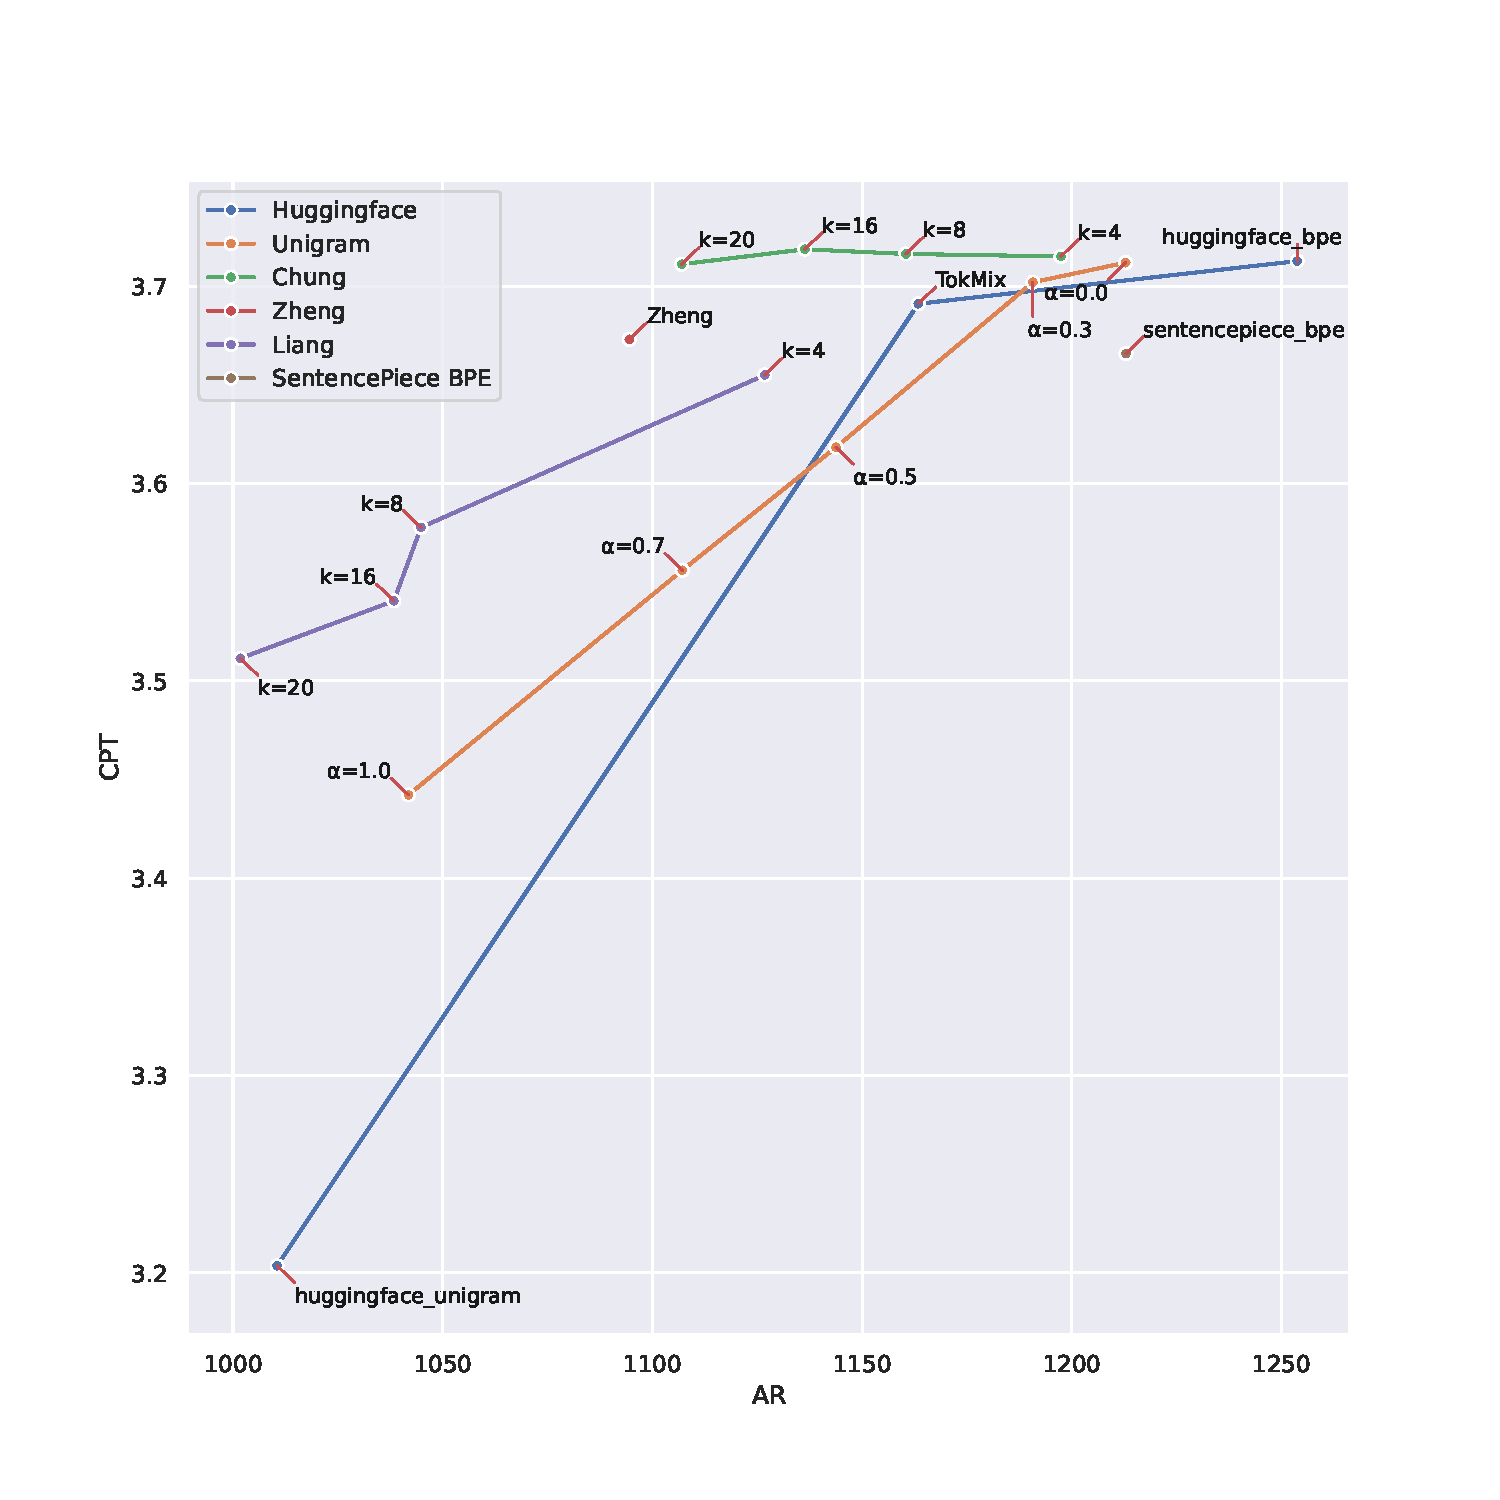
\includegraphics[width=\textwidth]{figures/all_tokenizers_AR_vs_CPT.pdf}
    \caption{We visualize the overall vocabulary allocation metrics for all tokenizers from Table \ref{tab:all_tokenizers_metrics}. We observe that the vocabulary allocation scores are related --- higher AR usually means higher CPT.  We also observe that Huggingface Unigram is a clear outlier, although a combination of separate, monolingual Huggingface Unigrams (TokMix) approaches the performance of the Sentencepiece Unigram with the corresponding data imbalance ($\alpha=0.3$). We see that the balancing methods overperform the unbalanced Unigrams ($\alpha=1.0$, $\alpha=0.7$) in terms of CPT but perform similarly or worse to the simple case of running the Sentencepiece Unigram trainer on a balanced set $\alpha=0.0$.}
    \label{fig:all_tokenizers_AR_vs_CPT}
\end{figure}

Crucially, we see that the reproduced methods of \citet{chung_improving_2020,zheng_allocating_2021,liang_xlm-v_2023} do improve over the unbalanced baselines $\alpha=1.0, 0.7, 0.5$ on the CPT metric, especially with a higher number of clusters. On the other hand, they do not outperform the simple case of training the Sentencepiece Unigram on a balanced dataset $\alpha=0.0$. We also observe that the clustering methods with a higher number of clusters along with Zheng are close to each other on the CPT-AR plot. We assume this is because, with higher $k$, the clustering methods reduce to the Zheng method (training separate tokenizers for each language). Similarly, with a lower number of clusters, the methods are much closer to the vanilla Sentencepiece Unigram $\alpha=1.0$ trained on the unbalanced dataset. We hypothesize that with a low amount of clusters, the original data imbalance starts to degrade performance for low-resource languages inside the clusters.

\begin{figure}
    \centering
    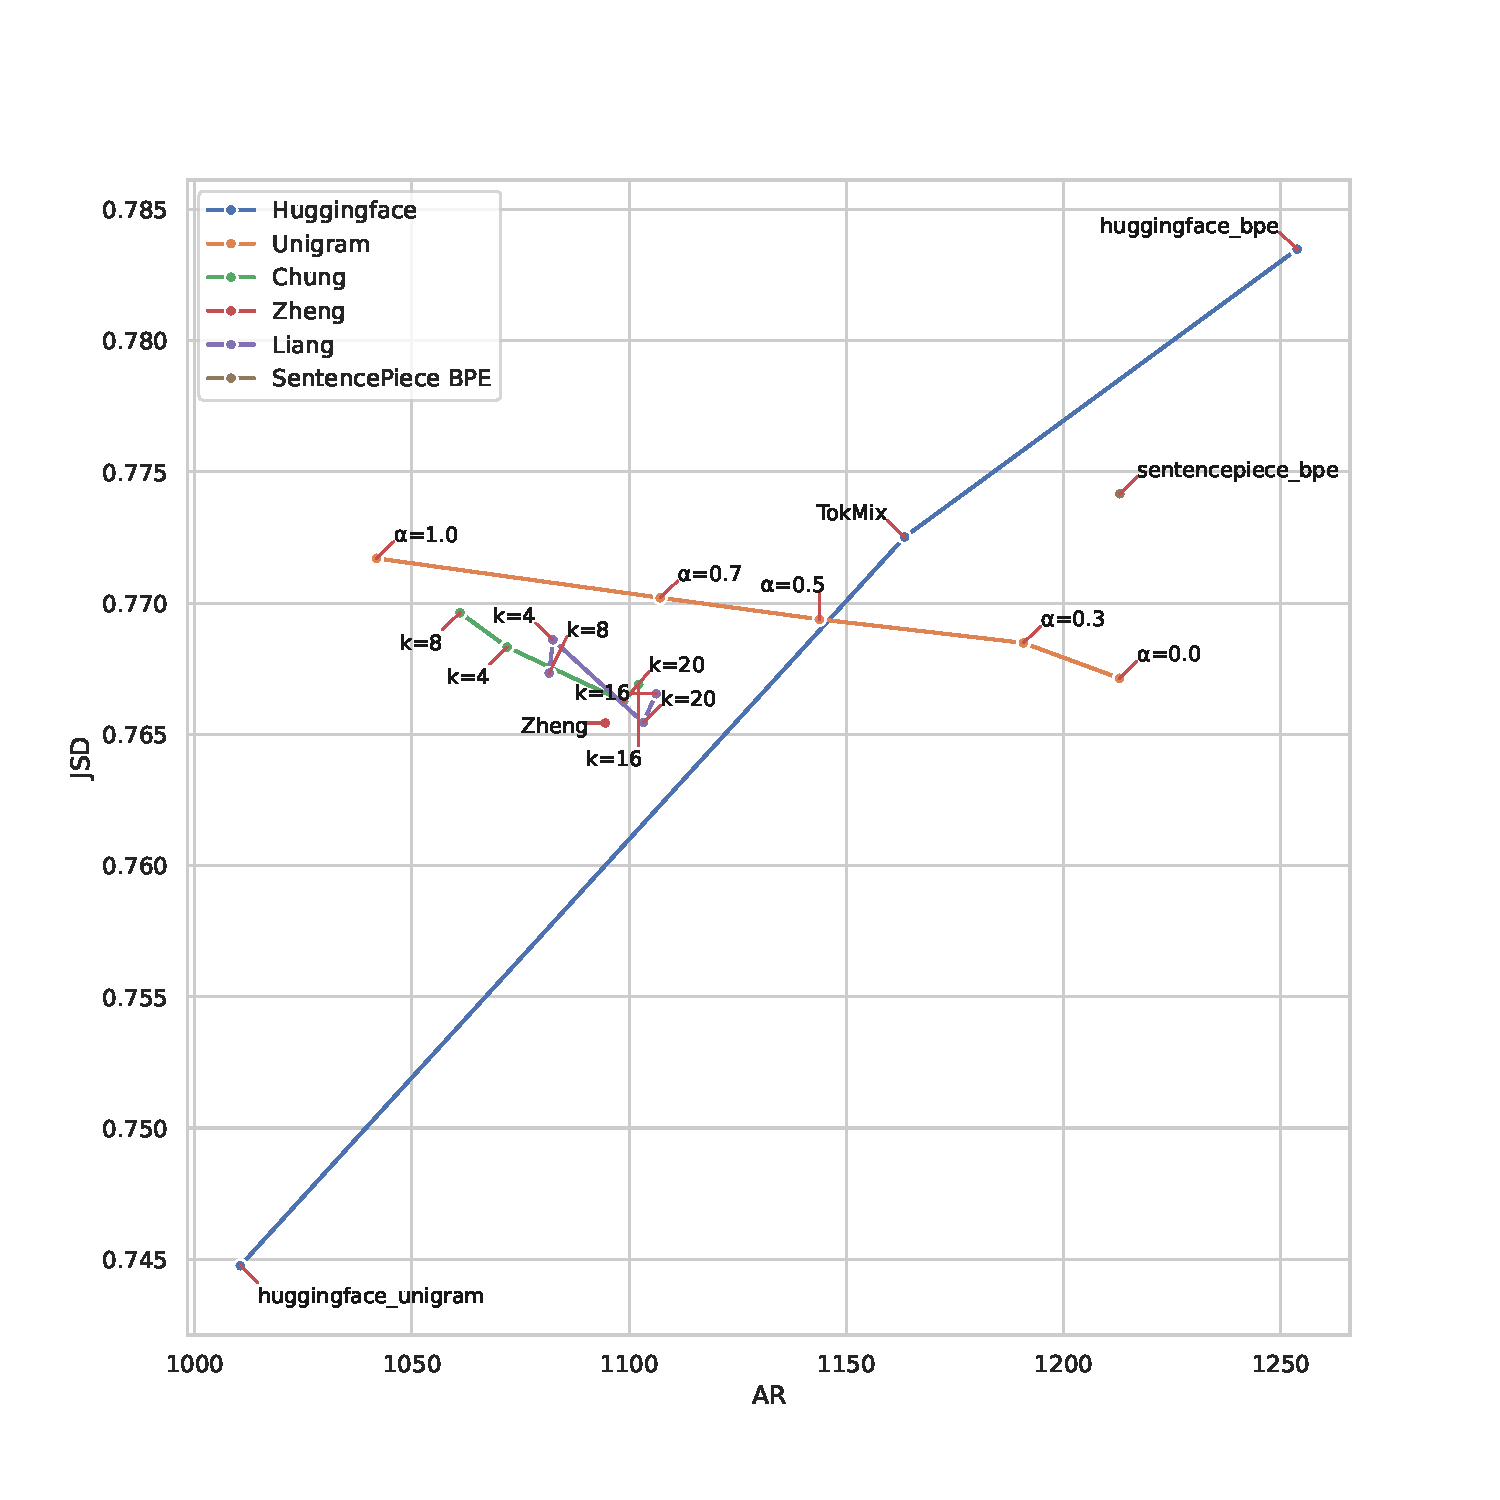
\includegraphics[width=\textwidth]{figures/all_tokenizers_AR_vs_JSD.pdf}
    \caption{We visualize the tokenizers from Table \ref{tab:all_tokenizers_metrics} in terms of Average Rank and Jensen-Shannon Divergence. Here we can see that all methods based on Sentencepiece result in similar overlap independent of the allocation. This is interesting because the replicated balancing methods (Chung, Zheng, Liang) work by splitting the data and training separate tokenizers. Nevertheless, after merging the separate subtokenizers they all seem to end up with similar vocabulary overlaps. The highest vocabulary isolation is surprisingly achieved by the Huggingface BPE tokenizer, which is contrary to the hypothesis stated by \citet{chung_improving_2020,zheng_allocating_2021} that the tokenizers trained on the concatenation of all data tend to select subwords shared across all languages.}
    \label{fig:all_tokenizers_AR_vs_JSD}
\end{figure}

We also explore the relationship between vocabulary allocation and vocabulary overlap on the \autoref{fig:all_tokenizers_AR_vs_JSD}. We see that the differences between all methods based on Sentencepiece are small compared to the differences between Huggingface tokenizers. This is surprising because the assumption shared by all authors of the balancing methods is that by training separate tokenizers, we achieve lower overlap between unrelated languages. Nevertheless, we see that the overall overlap is largely similar and more influenced by the choice of implementation. 

If we ignore the Huggingface outliers and interpret only the differences in the overlap between the balancing methods, we still see a counterintuitive trend where the Zheng method and a higher number of clusters have a \textit{larger overlap in vocabulary between languages} (lower JSD) than the standard tokenizers and clustering methods with lower number of clusters.
% This is surprising because one of the motivations for the method of Chung and Liang is to promote overlap between similar languages while minimizing the overlap between distant languages. We would therefore expect the overall overlap to decrease, as the number of spurious token sharing decreases. Nevertheless, we observe that the resulting overlap is lower or similar to our Sentencepiece Unigram tokenizers. Similarly, the Zheng method works by training separate tokenizers for each language and then combining them into one. We would expect the overlap to be even lower than the original Sentencepiece Unigram but we observe that the overlap is comparable. 
% Surprisingly, the lowest vocabulary overlap (highest JSD) is achieved by the Huggingface BPE trained on a combined corpus. 

\begin{figure}
    \centering
    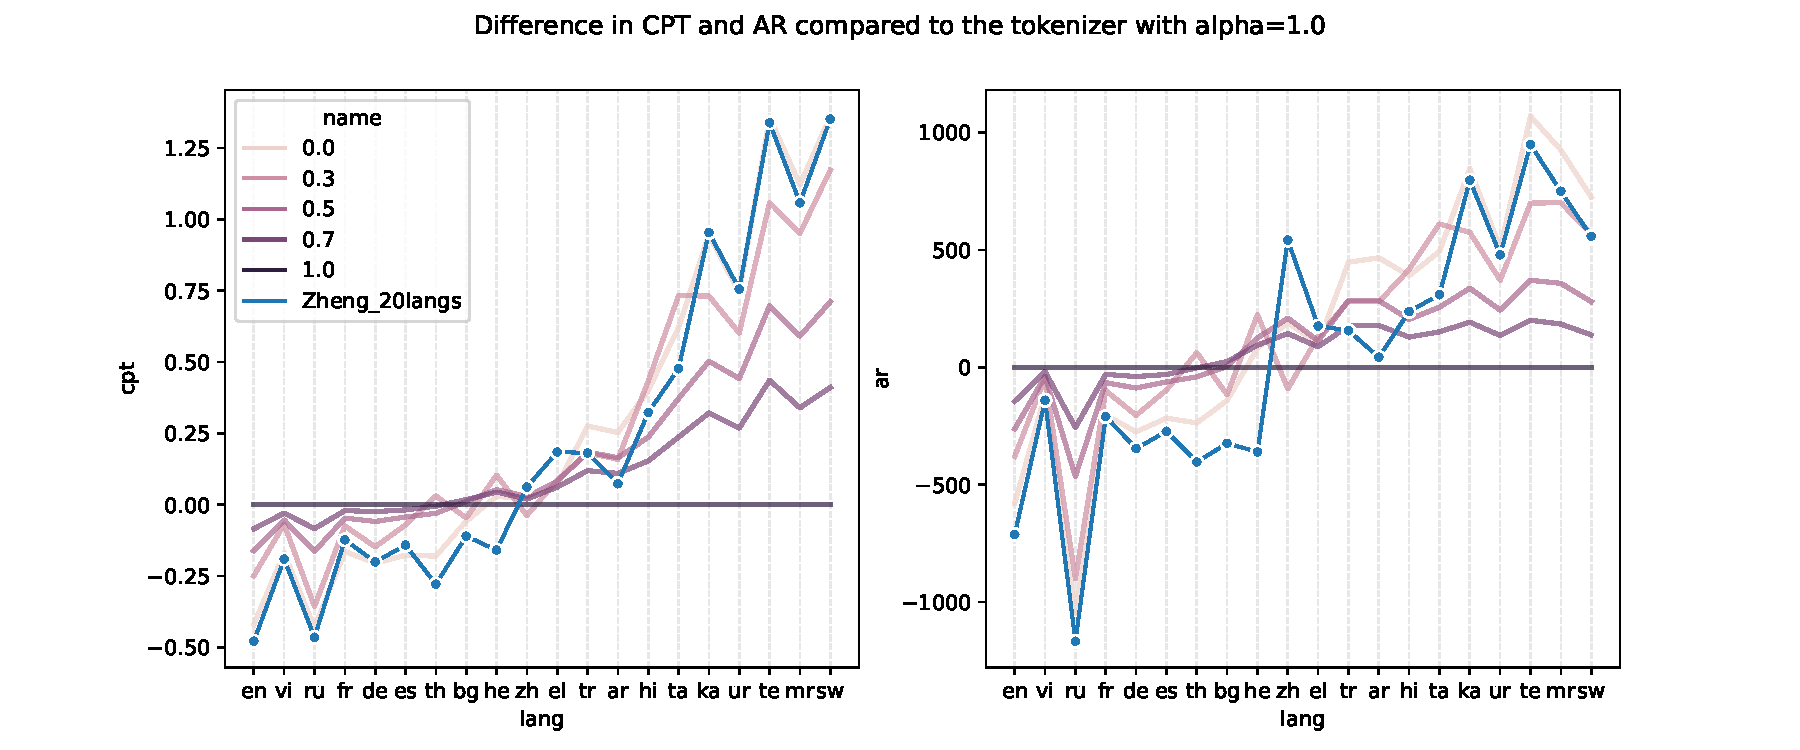
\includegraphics[width=\textwidth]{figures/zheng_vs_alphas.pdf}
    \caption{We zoom into the results of the Zheng method and compare the vocabulary allocation across the individual languages represented by this tokenizer against the backdrop of the vanilla Unigram tokenizers trained with different data imbalances from \ref{fig:data_balance_vs_allocation_per_lang}. We observe a striking similarity between the vocabulary allocation of the Zheng tokenizer and the Unigram tokenizer with $\alpha=0.0$, especially in terms of characters per token. This comes as a large surprise because the Zheng method works by training a separate tokenizer for each language and then merging them. Despite the different methods of obtaining the vocabulary, the resulting tokenizers are very similar across the languages.}
    \label{fig:zheng_vs_alphas}
\end{figure}

\subsection{Comparison of balancing methods per language}
\label{sec:comparison_balancing_methods_per_lang}

We investigate the differences between the balanced Unigram and the replicated methods in more detail by examining the CPT and AR metrics computed \textbf{per language}. This way we can better assess (\textbf{Q4}) how the methods improve the low-resource languages. We also more closely compare (\textbf{Q5}) the balancing methods with the Unigram tokenizers trained on different data imbalances. We do this by plotting only the differences per language between the methods and the Unigram tokenizer with the highest imbalance $\alpha=1.0$ similar to what we did in \autoref{fig:data_balance_vs_allocation_per_lang}.

We start by comparing the Zheng method with the increasingly imbalanced Unigram tokenizers in \autoref{fig:zheng_vs_alphas}. We plot the increase or decrease in vocabulary allocation metrics for each language sorted by the data available. Remarkably, we see that the Zheng method is strikingly similar in terms of CPT and AR per language to the Unigram tokenizer trained on the balanced set $\alpha=0.0$. The similarity seems to be higher in the CPT metric although the AR metric is also similar especially for the highest and lowest resource languages. We find this observation quite surprising because of the distinctness of the Zheng method --- it trains a separate tokenizer for each language and then merges the vocabularies together. Nevertheless, the resulting tokenizer is very similar to the Unigram tokenizer trained on the joint, balanced set. 

Intrigued by the similarity between the Zheng tokenizer and the Unigram tokenizer with $\alpha=0.0$, we also look at the differences in ALP metric which is used for the selection of vocabulary sizes in the Zheng method. In \autoref{fig:zheng_vs_alphas_alp} we see that the greedy optimization of ALP across languages indeed results in a similar vocabulary allocation as the Unigram tokenizer with $\alpha=0.0$.


\begin{figure}
    \centering
    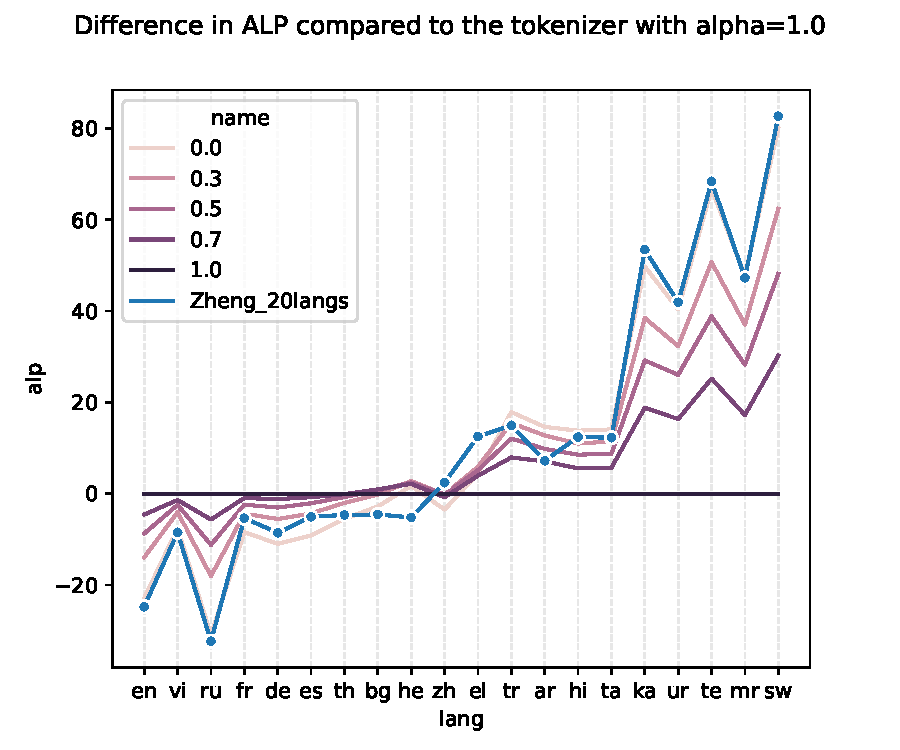
\includegraphics[width=0.5\textwidth]{figures/zheng_vs_alphas_alp.pdf}
    \caption{Intrigued by the similarity between the Zheng tokenizer and the Unigram tokenizer with $\alpha=0.0$ from Figure \ref{fig:zheng_vs_alphas} we also look at the ALP metric which is used for the selection of vocabulary sizes in the Zheng method. Here we see that the greedy optimization of ALP across languages indeed results in a similar vocabulary allocation as the Unigram tokenizer with $\alpha=0.0$.}
    \label{fig:zheng_vs_alphas_alp}
\end{figure}

\begin{figure}
    \centering
    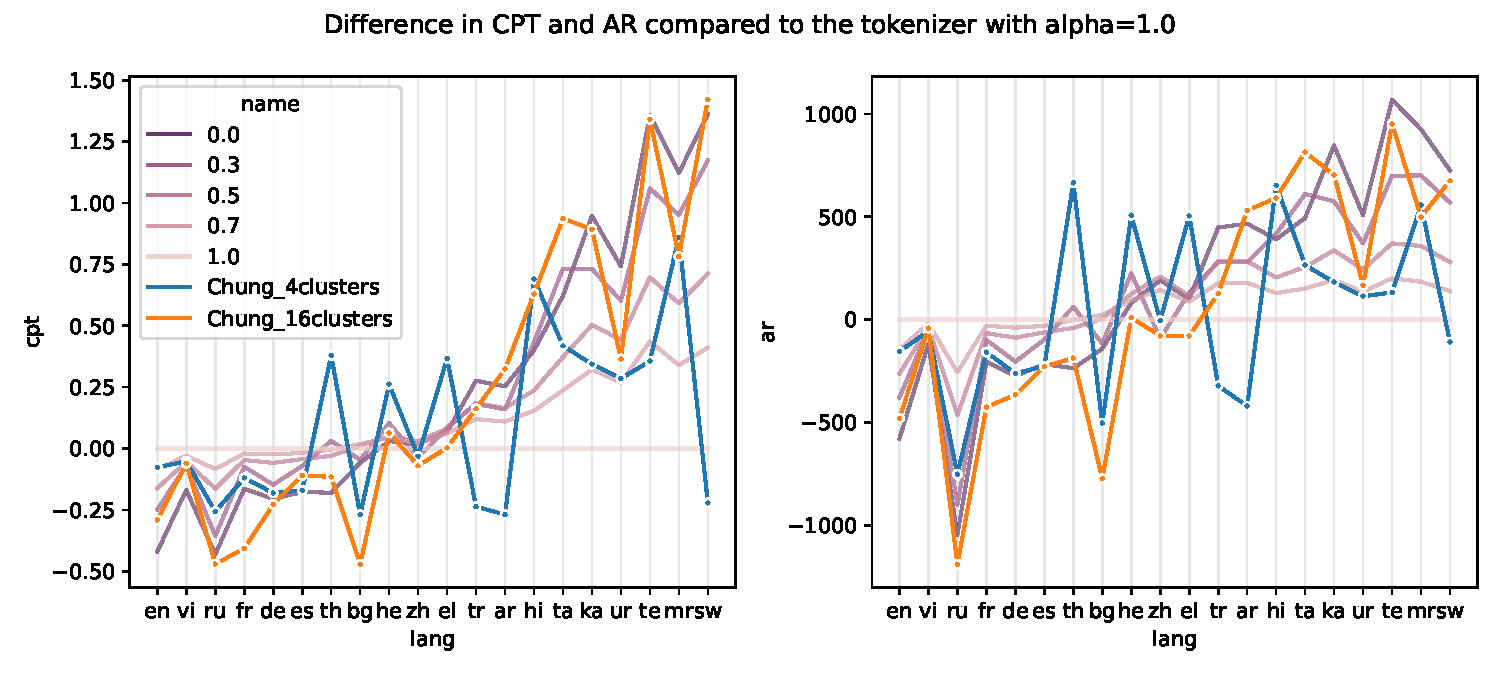
\includegraphics[width=\textwidth]{figures/chung_vs_alphas.pdf}
    \caption{Here we inspect the language-level vocabulary allocation of the Chung method. We see that the Chung method with higher number of clusters (k=16) resembles the Unigram tokenizer with $\alpha=0.0$ with large drops in allocation for Bulgarian (bg), Urdu (ur), Marathi(mr) and to a lesser degree French (fr). The lower number of clusters (k=4) differs more from the Unigram tokenizers. We see large increases in allocation for Thai (th), Hebrew (he), Greek (el), and Hindi (hi) and large decreases for Bulgarian (bg), Turkish (tr), Arabic (ar), and Swahili (sw).}
    \label{fig:chung_vs_alphas}
\end{figure}

Next, we inspect the Chung method and compare it in detail to our Unigram tokenizers in \autoref{fig:chung_vs_alphas}. For comparison, we select a run with a low number of clusters (k=4) and a high number of clusters (k=16). We see that the different numbers of clusters yield different results. In the case of a higher number of clusters, we see that the tokenizer exhibits a similar trend in CPT and AR across the languages as the balanced Unigram tokenizer with $\alpha=0.0$ albeit with some deviations. In the case of a lower number of clusters, the metrics per language seem to be more distinct compared to our Unigram tokenizers. 

We look at the CPT per language for k=16 more closely and identify the languages where the Chung tokenizer differs significantly from the Unigram tokenizer with $\alpha=0.0$. We see that the CPT drops significantly for Bulgarian (bg), Urdu (ur), Marathi (mr), and to some degree French (fr). On the other hand, we see smaller improvements for English (en), Vietnamese (vi), Spanish (es), Thai (th), Hindi (hi), and Tamil (ta). We compare this to the cluster assignments in \autoref{tab:chung_clusters_k16}. Revealingly, we observe that all languages with the large drop in CPT have been assigned to a cluster with another, higher-resource language. Bulgarian is assigned with Russian (8th largest corpus versus 3rd largest corpus), Urdu with Arabic (17th vs. 13th), Marathi with Hindu (18th vs. 14th) and French with English (4th vs. 1st). This seems to be in line with our hypothesis that inside clusters, the data imbalance may hurt the representation of low-resource languages.

We continue with a similar analysis for the 4 clusters. We see that the CPT for Bulgarian (bg), Turkish (tr), Arabic (ar), and Swahili (sw) is lower than any of our Unigram tokenizers. On the other hand, we see significant improvements for Thai (th), Hebrew (he), Greek (el), and Hindi (hi) over our Unigram tokenizers. Additionally, Marathi (mr) achieves the highest CPT increase over the unbalanced Unigram baseline, although the increase stays in the range of the $\alpha=0.5$ Unigram tokenizer. We again look at the cluster assignments in \autoref{tab:chung_clusters_k4}. We observe that Bulgarian and Arabic are assigned to a cluster with higher-resource Russian (3rd) and Chinese, which could explain the decrease in CPT for the two. Similarly, Swahili and Turkish which use the Latin script are assigned to a cluster with higher resource English (largest corpus) and Vietnamese (2nd largest). On the other hand, we see that Thai, Hebrew, and Greek are assigned to a cluster with lower-resource languages --- Tamil (ta), Georgian (ka), Urdu (ur), and Telugu (te). As we have observed, Thai, Hebrew, and Greek benefit from this assignment while the lower-resource languages seem to have a lower CPT than the $\alpha=0.7$ Unigram and therefore approach the unbalanced baseline.

\begin{figure}
    \centering
    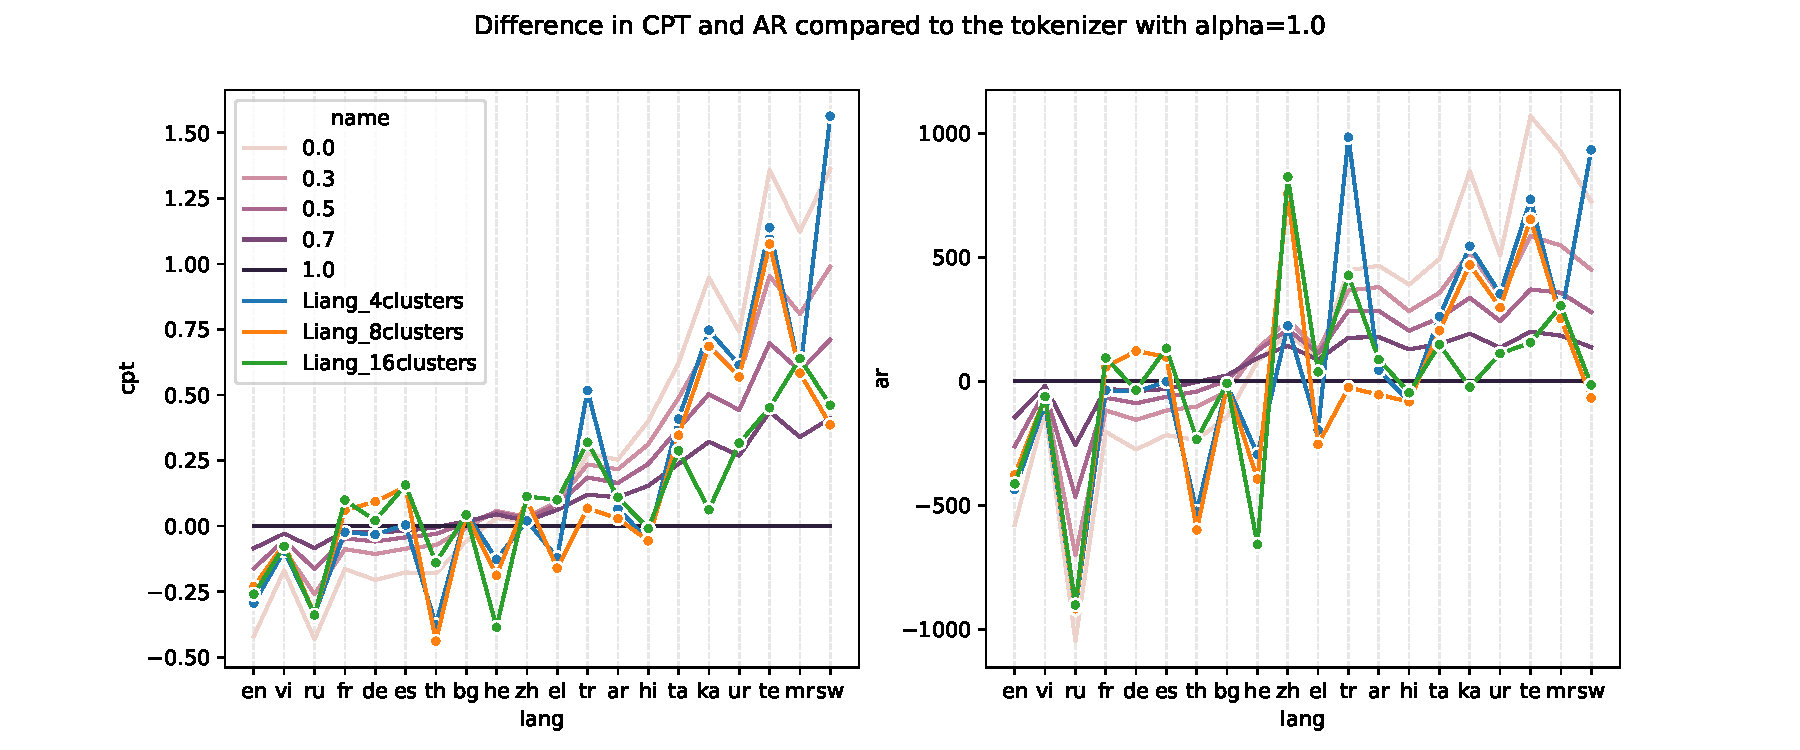
\includegraphics[width=\textwidth]{figures/liang_vs_alphas.pdf}
    \caption{We inspect the language-level vocabulary allocation of the Liang method. We see similarities to the Chung method in \autoref{fig:chung_vs_alphas}. The main differences seem to be the improved Chinese and Arabic for 4 clusters and worse Hebrew and better Urdu for 16 clusters. Overall the results are similar.}
    \label{fig:liang_vs_alphas}
\end{figure}

We look at the \citet{liang_xlm-v_2023} replication results in \autoref{fig:liang_vs_alphas}. We see that despite a slightly different clustering method and per-cluster vocabulary size selection, the Liang method exhibits similar patterns we observed in the Chung method.

Overall, we infer that the Chung and Liang methods are sensitive to cluster assignments. Because the training data are merged per cluster, if a low-resource language gets assigned to a cluster with a high-resource language, the language imbalance acts in favor of the high-resource language. As we know from our experiments in \autoref{sec:tokenizer_training_with_data_imbalance} presented previously, the benefit of adding more data to the high-resource language is lower than the cost that incurs on the low-resource language. We believe this is the cause of the lower overall CPT and AR for the clustering methods.

\subsection{Comparison of balancing methods on downstream tasks}

We validate our observations from the previous \autoref{sec:comparison_balancing_methods_per_lang} by evaluating the tokenizers extrinsically. We again address (\textbf{Q4}) and (\textbf{Q5}) and investigate the differences between the balancing methods and the Sentencepiece Unigram tokenizers. In this section, however, we focus on the actual influence of the tokenizers on the multilingual language models and assess the differences between tokenizers by the performance on downstream tasks.

We select the balancing methods by \citet{chung_improving_2020,zheng_allocating_2021}. For the clustering method, we select a low- and high- number of clusters $k=4\text{ and }16$. We compare the selected balancing tokenization methods to the standard Unigram tokenizers trained on differently balanced datasets with $\alpha=1.0, 0.3\text{ and }0.0$

\begin{figure}
    \centering
    \begin{subfigure}{.5\textwidth}
      \centering
      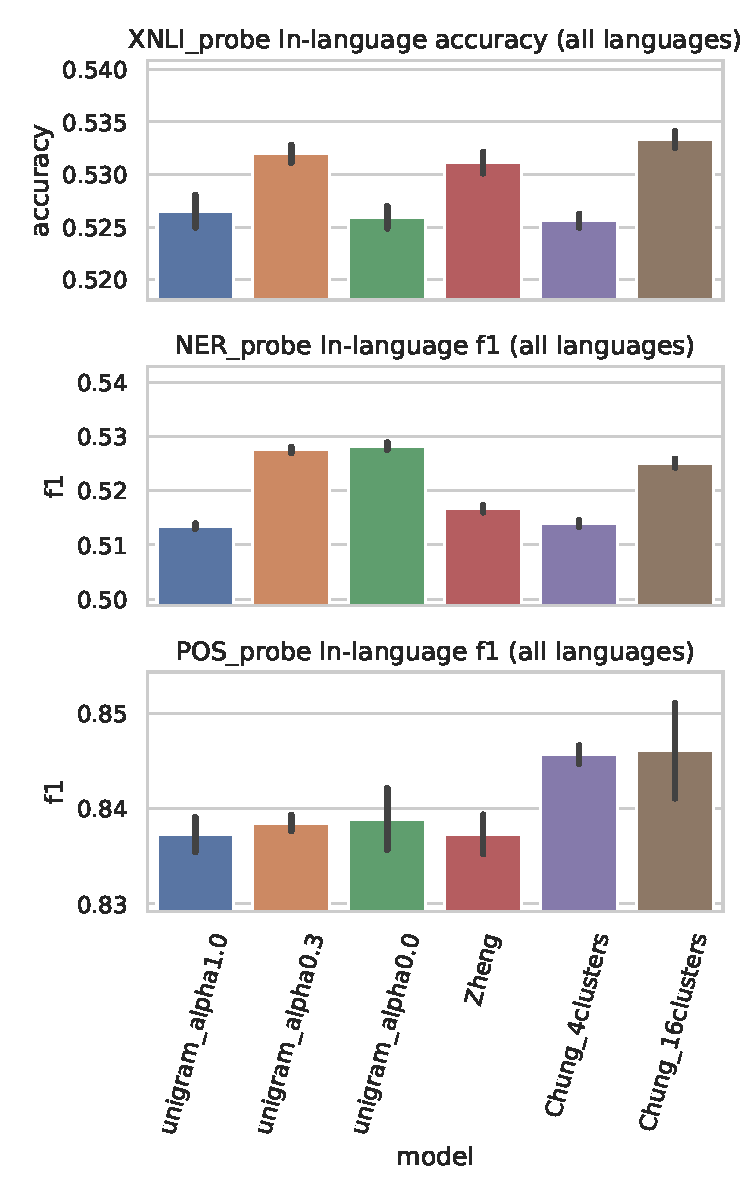
\includegraphics[width=\linewidth]{figures/probe_overall_inlanguage.pdf}
      \caption{In-language results}
      \label{fig:probe_overall_inlanguage}
    \end{subfigure}%
    \begin{subfigure}{.5\textwidth}
      \centering
      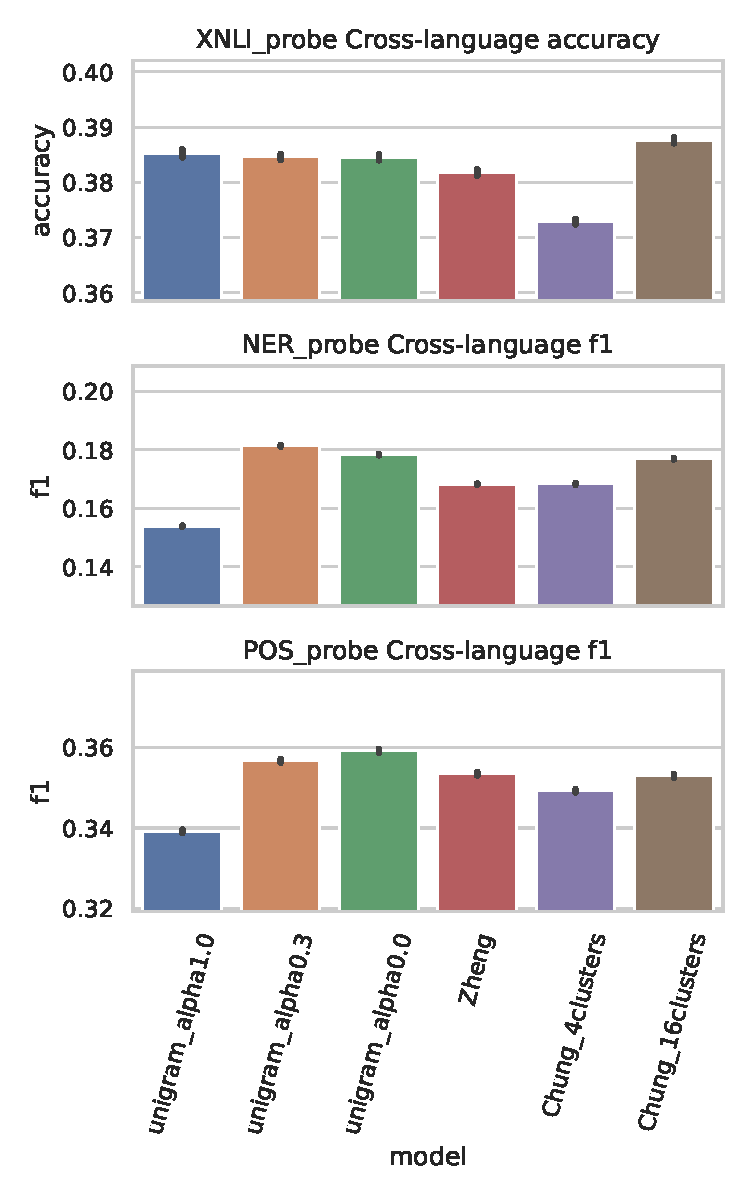
\includegraphics[width=\linewidth]{figures/probe_overall_crosslanguage.pdf}
      \caption{Cross-language results}
      \label{fig:probe_overall_crosslanguage}
    \end{subfigure}
    \caption{We select the replicated methods by \citet{chung_improving_2020,zheng_allocating_2021} and compare them with the vanilla Unigram tokenizers. For comparison, we choose the unbalanced Unigram tokenizer with $\alpha=1.0$ and then two stronger baselines with $\alpha=0.0$ and $\alpha=0.3$ trained on more balanced data. We then pretrain masked language models that differ only in the tokenizer they use and assess the performance of these models on the downstream tasks using probing. We test two settings --- in-language performance, where the model is trained on each of the available languages and then evaluated on the same language, and cross-language performance, where the model is also trained on each language but evaluated on all \textit{but} the training language. The results are a macro average over all the languages (in-language results) or all language pairs (cross-language results). For each model, language, and task we do 3 probe training runs with different random seeds. The error bars represent one standard deviation computed with bootstrapping by randomly sampling seeds for each language.}
    \label{fig:probe_overall}
\end{figure}

\subsubsection{Overall in-language and cross-language results}

In \autoref{fig:probe_overall}, we report the overall in-language and cross-language results for the models. We observe the clearest regularity in cross-language performance for word-level tasks (NER and POS), where all balancing methods and Unigram $\alpha=0.0,0.3$ improve over the unbalanced $\alpha=1.0$ model. Next, we see higher POS in-language scores for the Chung methods and higher NER in-language scores for the balanced unigrams ($\alpha=0.0\text{ and }0.3$). For in-language NLI, we do not see any systematic effect --- the differences between the models are small ($<1$ percentage point) and the outlier behavior of $\alpha=0.3$ compared to $\alpha=1.0\text{ and }0.0$ suggests that the variance is caused by the finetuning rather than any tokenizer effect.

\subsubsection{In-language and cross-language results examined by language}

We inspect the results more closely on the language level. We again compare the performance of the more balanced models to the unbalanced model by plotting the difference in accuracy and F1 score for the tasks by language. The languages are again sorted in descending order based on the amount of available data. 

\begin{figure}
    \centering
    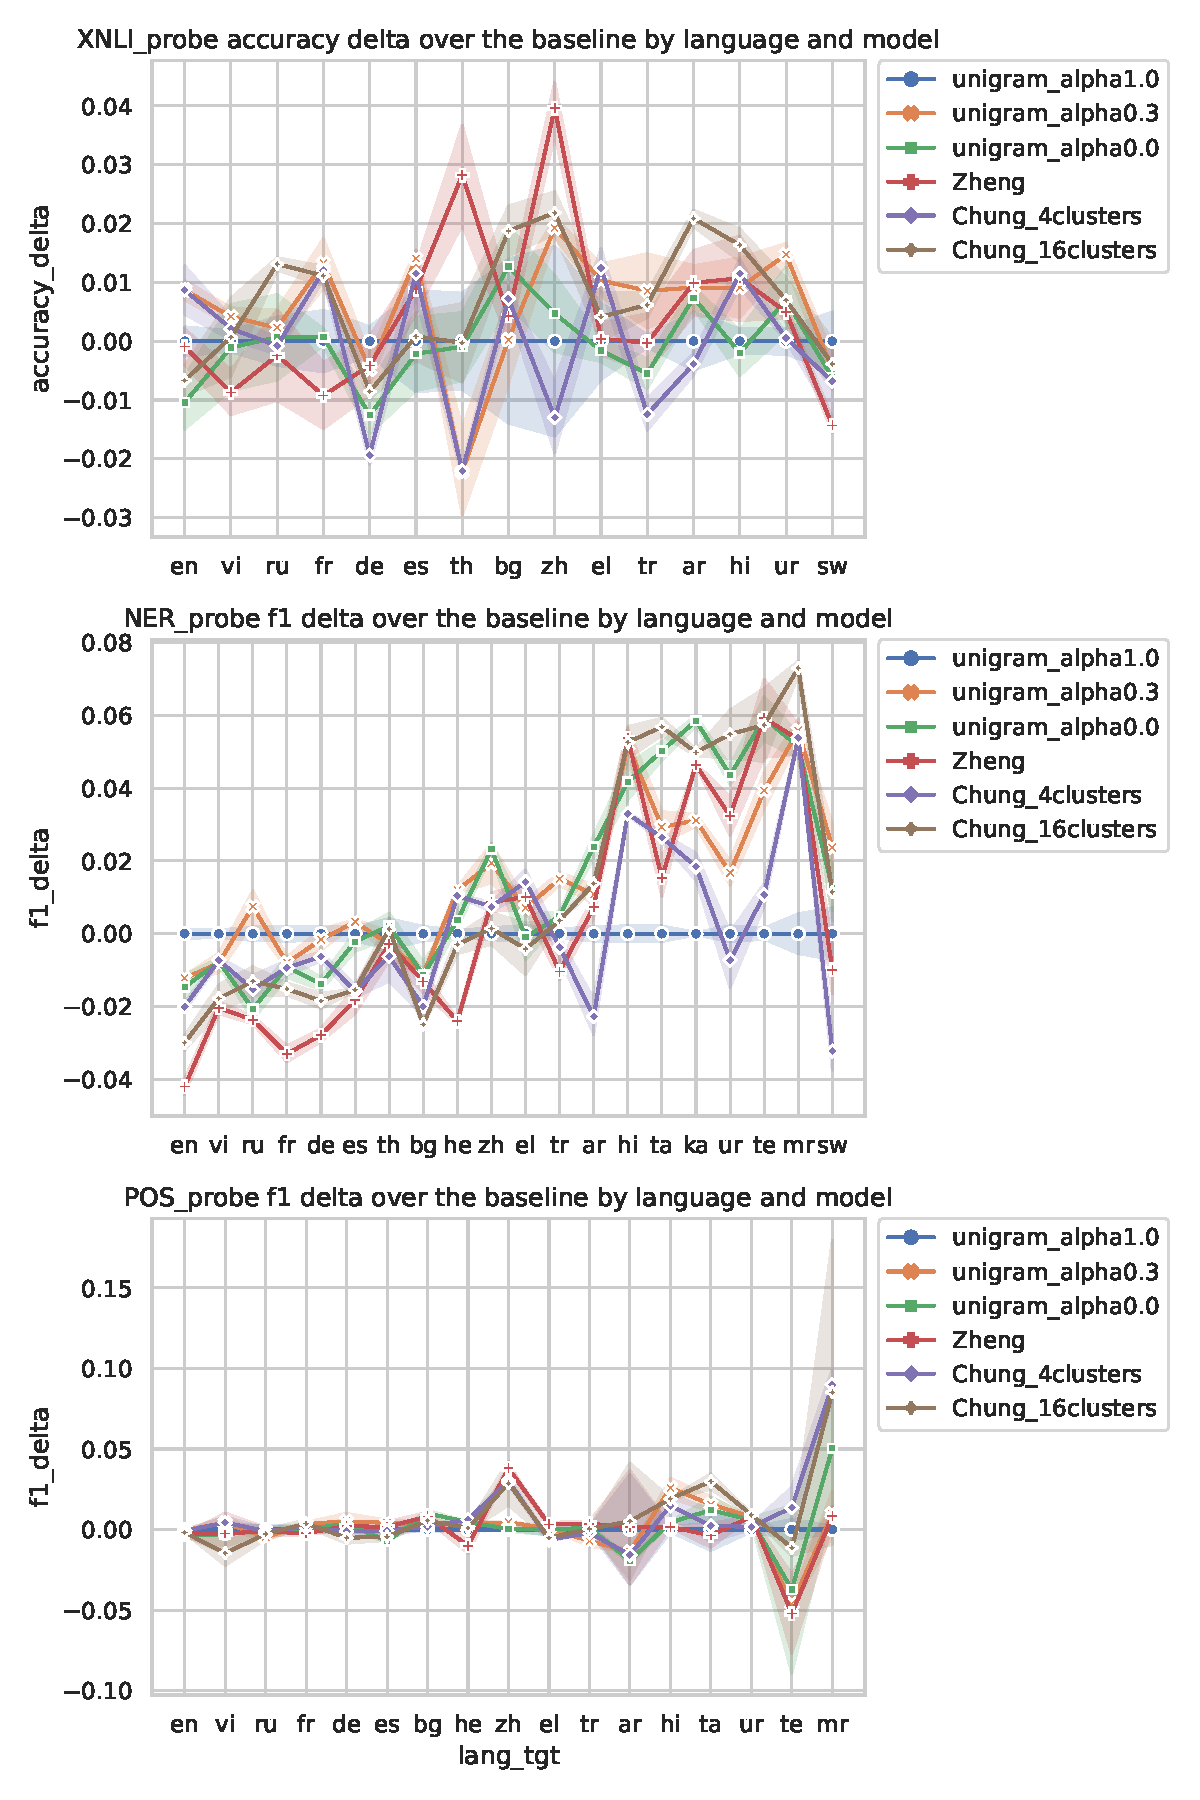
\includegraphics[width=0.8\textwidth]{figures/probe_detailed_inlanguage_over_baseline.pdf}
    \caption{We zoom in on the in-language results from Figure \ref{fig:probe_overall_inlanguage} and compare the performance of the balanced tokenizers against the unbalanced Unigram tokenizer with $\alpha=1.0$ over all tested languages for the tasks. In the case of the word-level tasks, especially in the case of named entity recognition, we observe a clear trend in line with our tokenizer investigations in \ref{fig:chung_vs_alphas}. The balancing methods improve the language representations for word-level tasks. For the sentence-level tasks, we do not observe any systematic effects. The error bands are one standard deviation computed from the three probe training runs with different random seeds.}
    \label{fig:probe_overall_inlanguage_over_baseline}
\end{figure}

In \autoref{fig:probe_overall_inlanguage_over_baseline}, we see the in-language results laid out by language. We see a large effect of the probe training language on the NER F1 score and to some degree an effect on the POS F1. We do not see a systematic effect on NLI. For NER, we see the effect of the tokenizer language balance reminiscent of the results in \autoref{fig:zheng_vs_alphas} and \autoref{fig:chung_vs_alphas}. For high-resource languages, we observe a decrease in performance across the board. This is counterbalanced by a larger increase in performance for the low-resource languages. This effect seems to be largest for the $\alpha=0.0$ Unigram tokenizer, Zheng method and Chung with 16 clusters. For $\alpha=0.3$ Unigram and Chung with 4 clusters, we see a similar effect but with a smaller magnitude, which is in line with our previous observations in \autoref{fig:chung_vs_alphas} in the intrinsic evaluation. In the case of POS, we do see more variance in results towards the low-resource languages but the effect is not as clear as for NER. We see significant improvements with Zheng and Chung methods on Chinese which correspond to the AR improvement for Chinese for the Zheng method in \autoref{fig:zheng_vs_alphas} but we do not see any difference in Chinese tokenizer metrics in the case of Chung (\autoref{fig:chung_vs_alphas}). We also see some improvements in Hindi, Tamil, and Marathi. For Telugu, we see a surprising drop for all methods except Chung with 4 clusters. % Note that the variance in the results is larger for the low-resource languages because of smaller test sets.


\begin{figure}
    \centering
    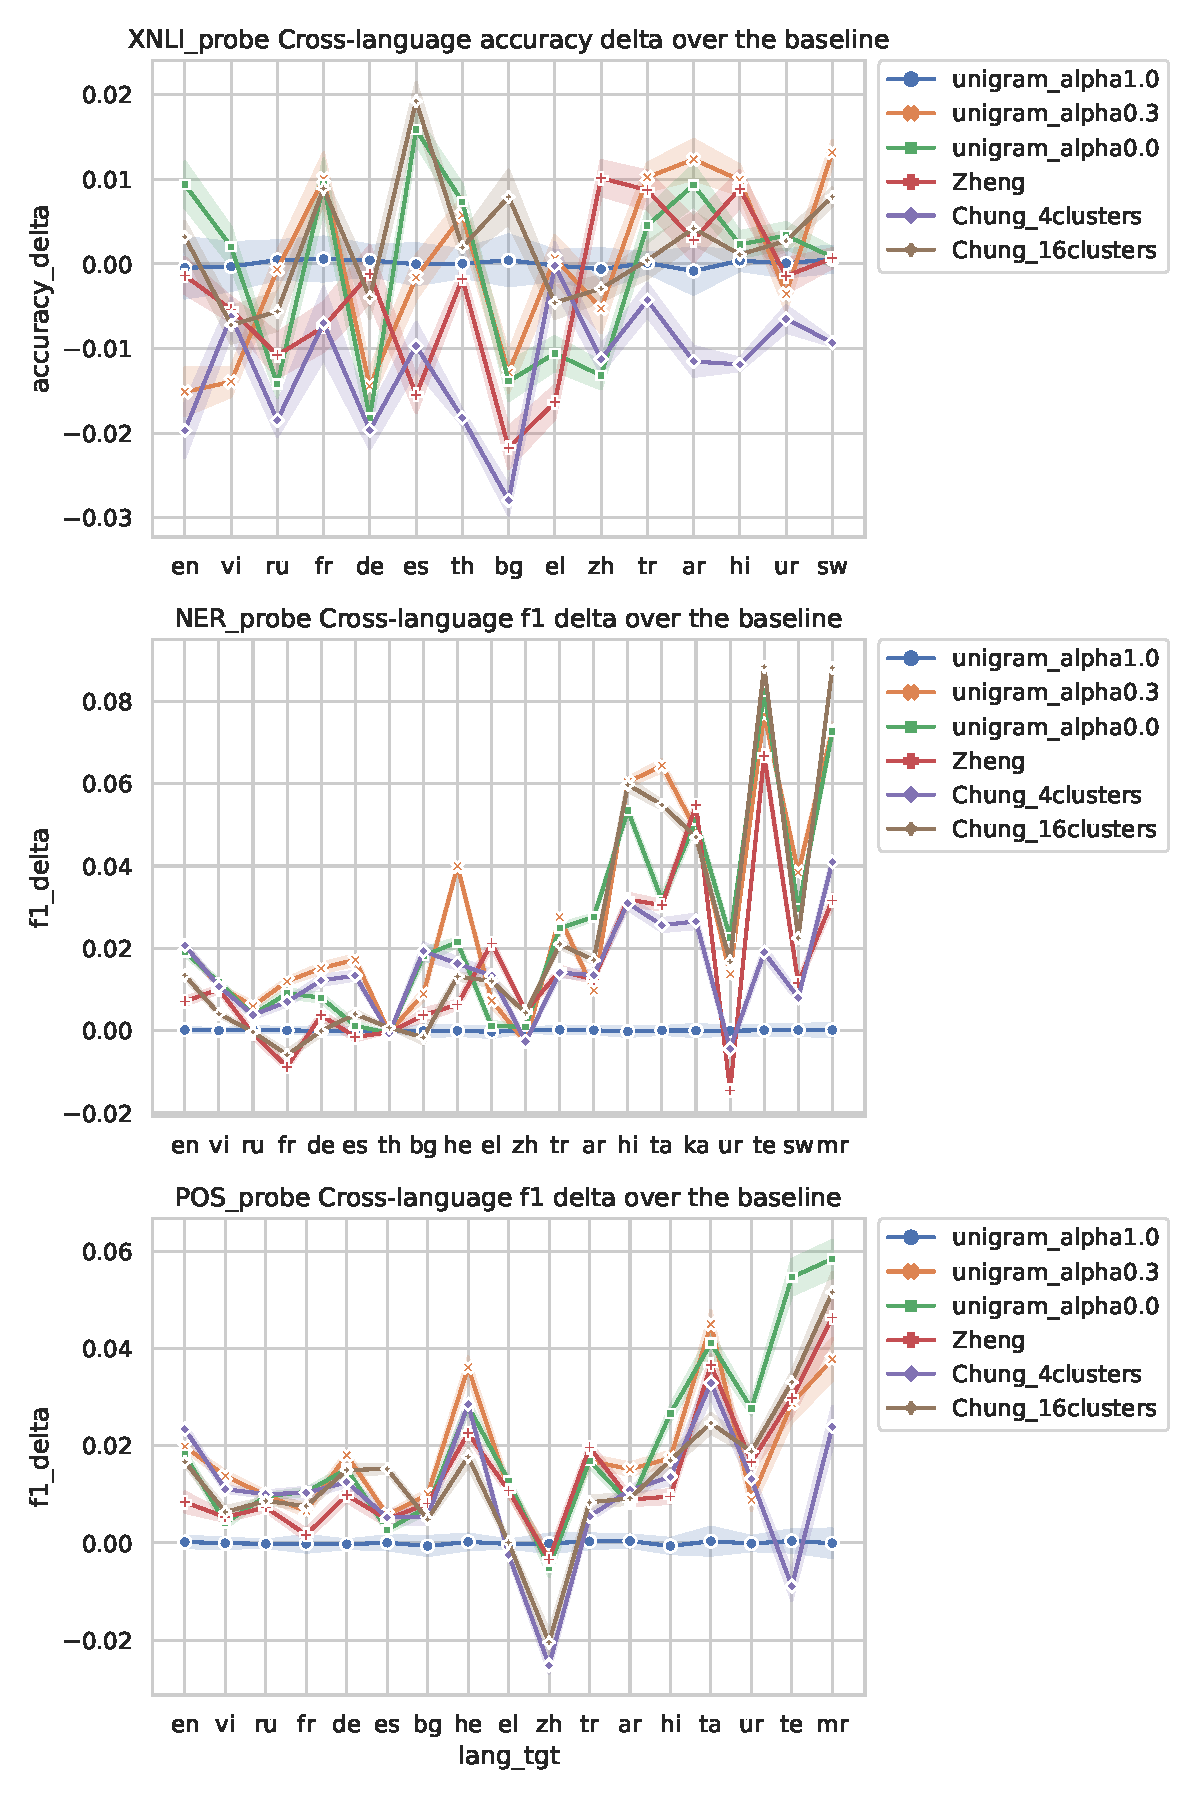
\includegraphics[width=0.8\textwidth]{figures/probe_detailed_crosslanguage_over_baseline_lang_tgt.pdf}
    \caption{Here we investigate in detail the cross-lingual results from Figure \ref{fig:probe_overall_crosslanguage} with comparison to the unbalanced Unigram tokenizer with $\alpha=1.0$. We observe that word-level task transfers behave in line with the tokenizer investigations in \ref{fig:chung_vs_alphas}. Moreover, it seems that both high-resource and low-resource languages benefit from the balancing methods, although the change is most clear on the low-resource side. For the sentence-level tasks, we do not observe any systematic effects. The value for each language and model is computed by averaging the difference in cross-lingual performance for the given \textit{target} language over the baseline. }
    \label{fig:probe_overall_crosslanguage_over_baseline}
\end{figure}

We turn our attention to the cross-language results in \autoref{fig:probe_overall_crosslanguage_over_baseline}. Here we again do not see any patterns in the NLI task, other than an overall drop in performance for Chung with 4 clusters, for which we do not have an explanation. On the other hand, we see clear patterns in NER and POS tasks. For both tasks, we see that the performance for low-resource languages is improved over the unbalanced baseline. Moreover, we see that the balancing has a net positive effect even for the high-resource languages, although the effect is not as pronounced as for the low-resource languages. In the NER task, we see that the Chung method with 4 clusters does not seem to improve on low-resource language as much as the other methods. 

\subsubsection{Direct comparison between intrinsic and extrinsic metrics}

Lastly, we plot the differences in tokenizer metrics against the differences in downstream task scores in scatter matrices. This allows us to directly compare the relationship between intrinsic tokenizer metrics and downstream performance.

In \autoref{fig:probe_overall_inlanguage_scattermatrix} we show the in-language results and in \autoref{fig:probe_overall_crosslanguage_scattermatrix} we show the cross-language results. 

In the case of in-language results, we see that for the NER and POS tasks, there is a significant Spearman correlation between the differences in tokenizer metrics and the differences in task performance (0.84 and 0.34 Spearman correlation respectively). For the NLI task, we do not observe any significant correlations. This is in line with our observations from the language-level results (\autoref{fig:probe_overall_inlanguage_over_baseline}). 

In the case of cross-language results, we observe significant, low, negative Spearman correlations between JSD and word-level tasks NER and POS (-0.21 and -0.22 respectively). We also see significant correlations between combined CPT/AR and all downstream tasks (0.14 for NLI, 0.39 for NER, and 0.29 for POS). The negative correlation between JSD and word-level tasks is at odds with our finding in \autoref{chap:experiment_1_validity} and supports our hypothesis that the correlation between JSD and downstream performance is confounded by the vocabulary allocation. The positive correlation between CPT/AR and downstream performance is in line with our findings in \autoref{chap:experiment_1_validity} and suggests that the downstream performance is positively influenced by the increase in token length in source and target languages. \footnote{A possible explanation of the contradictory findings of the JSD influence may be observed in the summary plot \autoref{fig:all_tokenizers_AR_vs_JSD}. We see that in our first batch of Huggingface experiments JSD correlates positively with AR, on the other hand the current batch of experiments shows a negative correlation.}

\subsubsection{Conclusion of the extrinsic evaluation}

Collecting all our observations together, we see that the tokenizers that aim to balance low-resource and high-resource languages do influence the results of downstream tasks compared to an unbalanced tokenizer. We see that the effect varies by task and language. 

Generally, we see a high influence on word-level tasks (NER and POS) and no significant influence on NLI. The effect of balancing is most prominent for in-language NER and cross-language NER and POS. Interestingly, in cross-language, the balancing effect is a net positive even for the high-resource languages.

For all cases where the balancing effect is clear (NER in-language, NER/POS cross-language), the best overall performance is achieved by the Unigram tokenizer trained on a balanced train set with $\alpha=0.0\text{ and }0.3$ (\autoref{fig:probe_overall}).

%In the case of in-language results, the effect of increasing the vocabulary allocation for low-resource languages and decreasing allocation for high-resource languages is clear for the NER task (\autoref{fig:probe_overall_inlanguage_over_baseline}). In the case of cross-lingual transfer, this effect is clear on both word-level tasks and, interestingly, is a net positive even for the high-resource tasks (\autoref{fig:probe_overall_crosslanguage_over_baseline}). For all cases where the balancing effect is clear (NER in-language, NER/POS cross-language), the best overall performance is achieved by the Unigram tokenizer trained on a balanced train set with $\alpha=0.0\text{ and }0.3$ (\autoref{fig:probe_overall}). For in-language POS, we see the best performance for the Chung method. To quantify the strength of the influence of tokenizer improvement on task improvement, we plot the metrics and downstream results in a scatterplot matrix and compute Spearman correlations between them. For all cases where the balancing effect is clear, we see significant correlations between the differences in tokenizer metrics and the differences in downstream task performance (\autoref{fig:probe_overall_inlanguage_scattermatrix} and \autoref{fig:probe_overall_crosslanguage_scattermatrix}). In general, the correlations we observe suggest that improving vocabulary allocation (CPT, AR) has a positive effect on in-language and cross-language performance on word-level tasks. Moreover, higher vocabulary overlap (lower JSD) also seems to have a positive effect on word-level tasks, although the effect is smaller. 
% Moreover, we also observe significant correlations between inlanguage POS and CPT/AR and significant, low correlation between crosslanguage NLI and CPT/AR

\begin{figure}
    \centering
    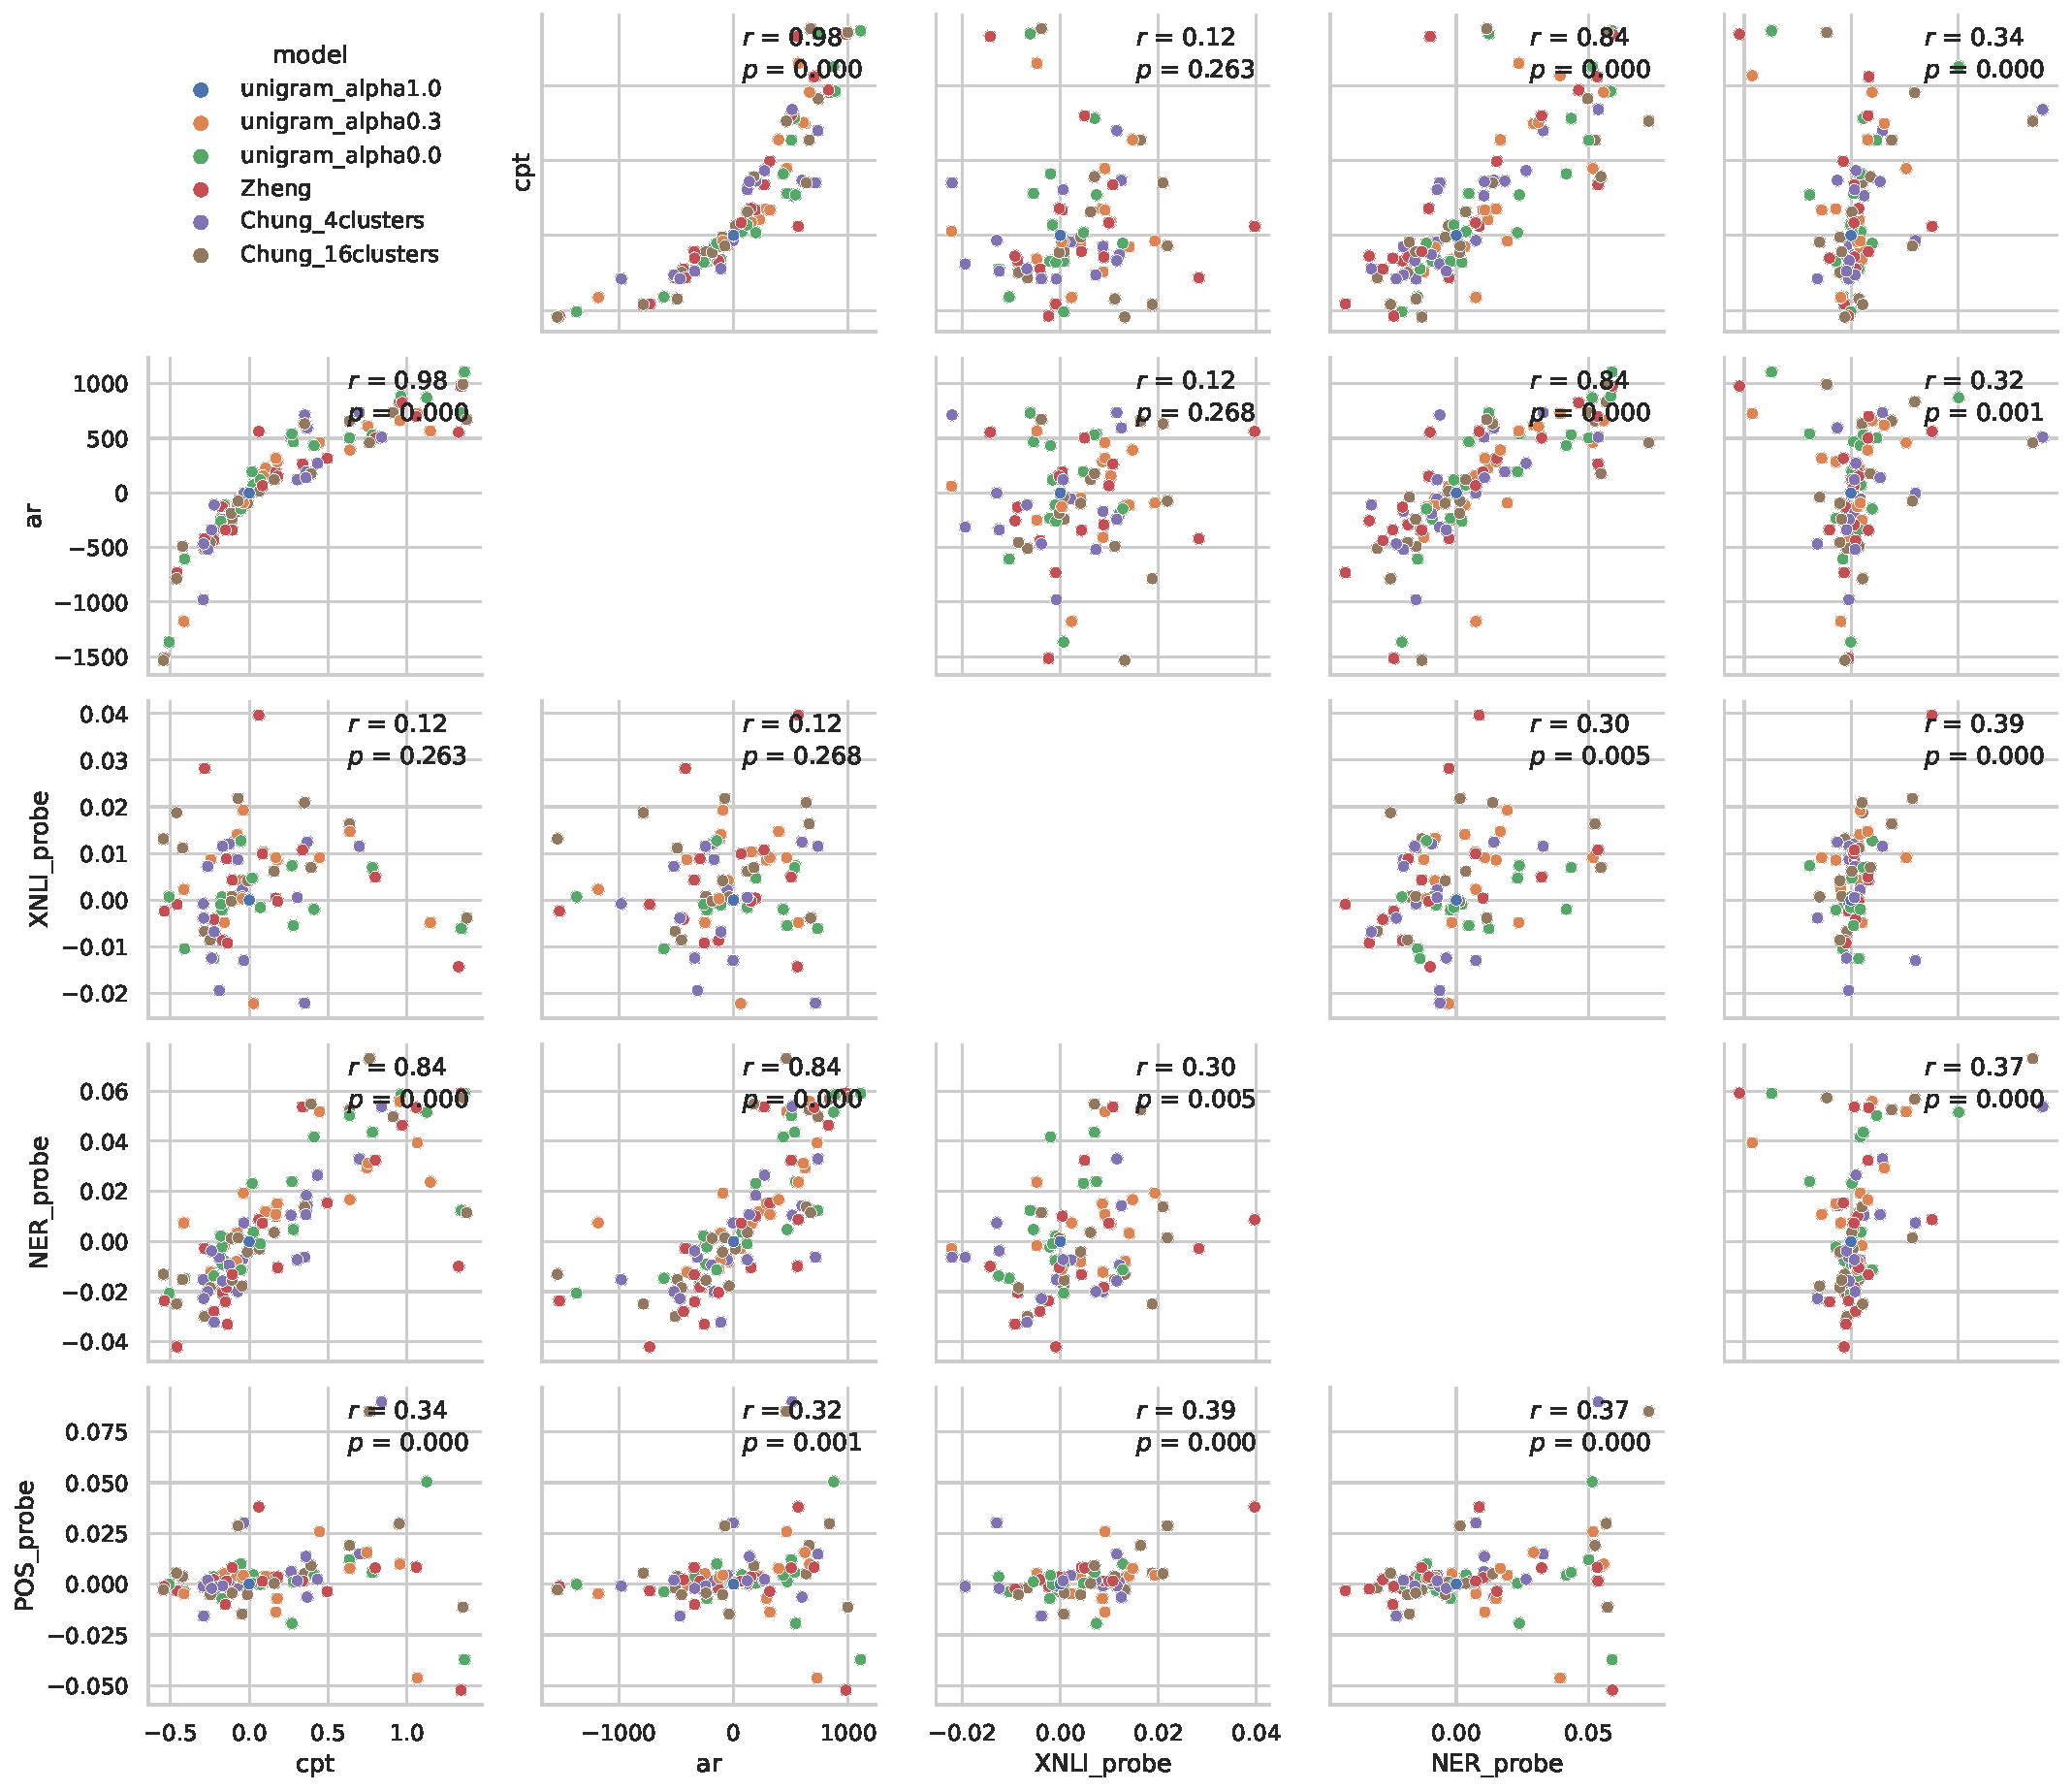
\includegraphics[width=\textwidth]{figures/probe_detailed_inlanguage_scattermatrix.pdf}
    \caption{We visualize the in-language results from Figure \ref{fig:probe_overall_inlanguage} in a scatter matrix. We substract mean result across three tokenization mwethods from per-language results. We see significant Spearman correlations for the NER and POS tasks, although for POS the correlation is low. For the NLI task, we do not observe any significant correlations.}
    \label{fig:probe_overall_inlanguage_scattermatrix}
\end{figure}

\begin{figure}
    \centering
    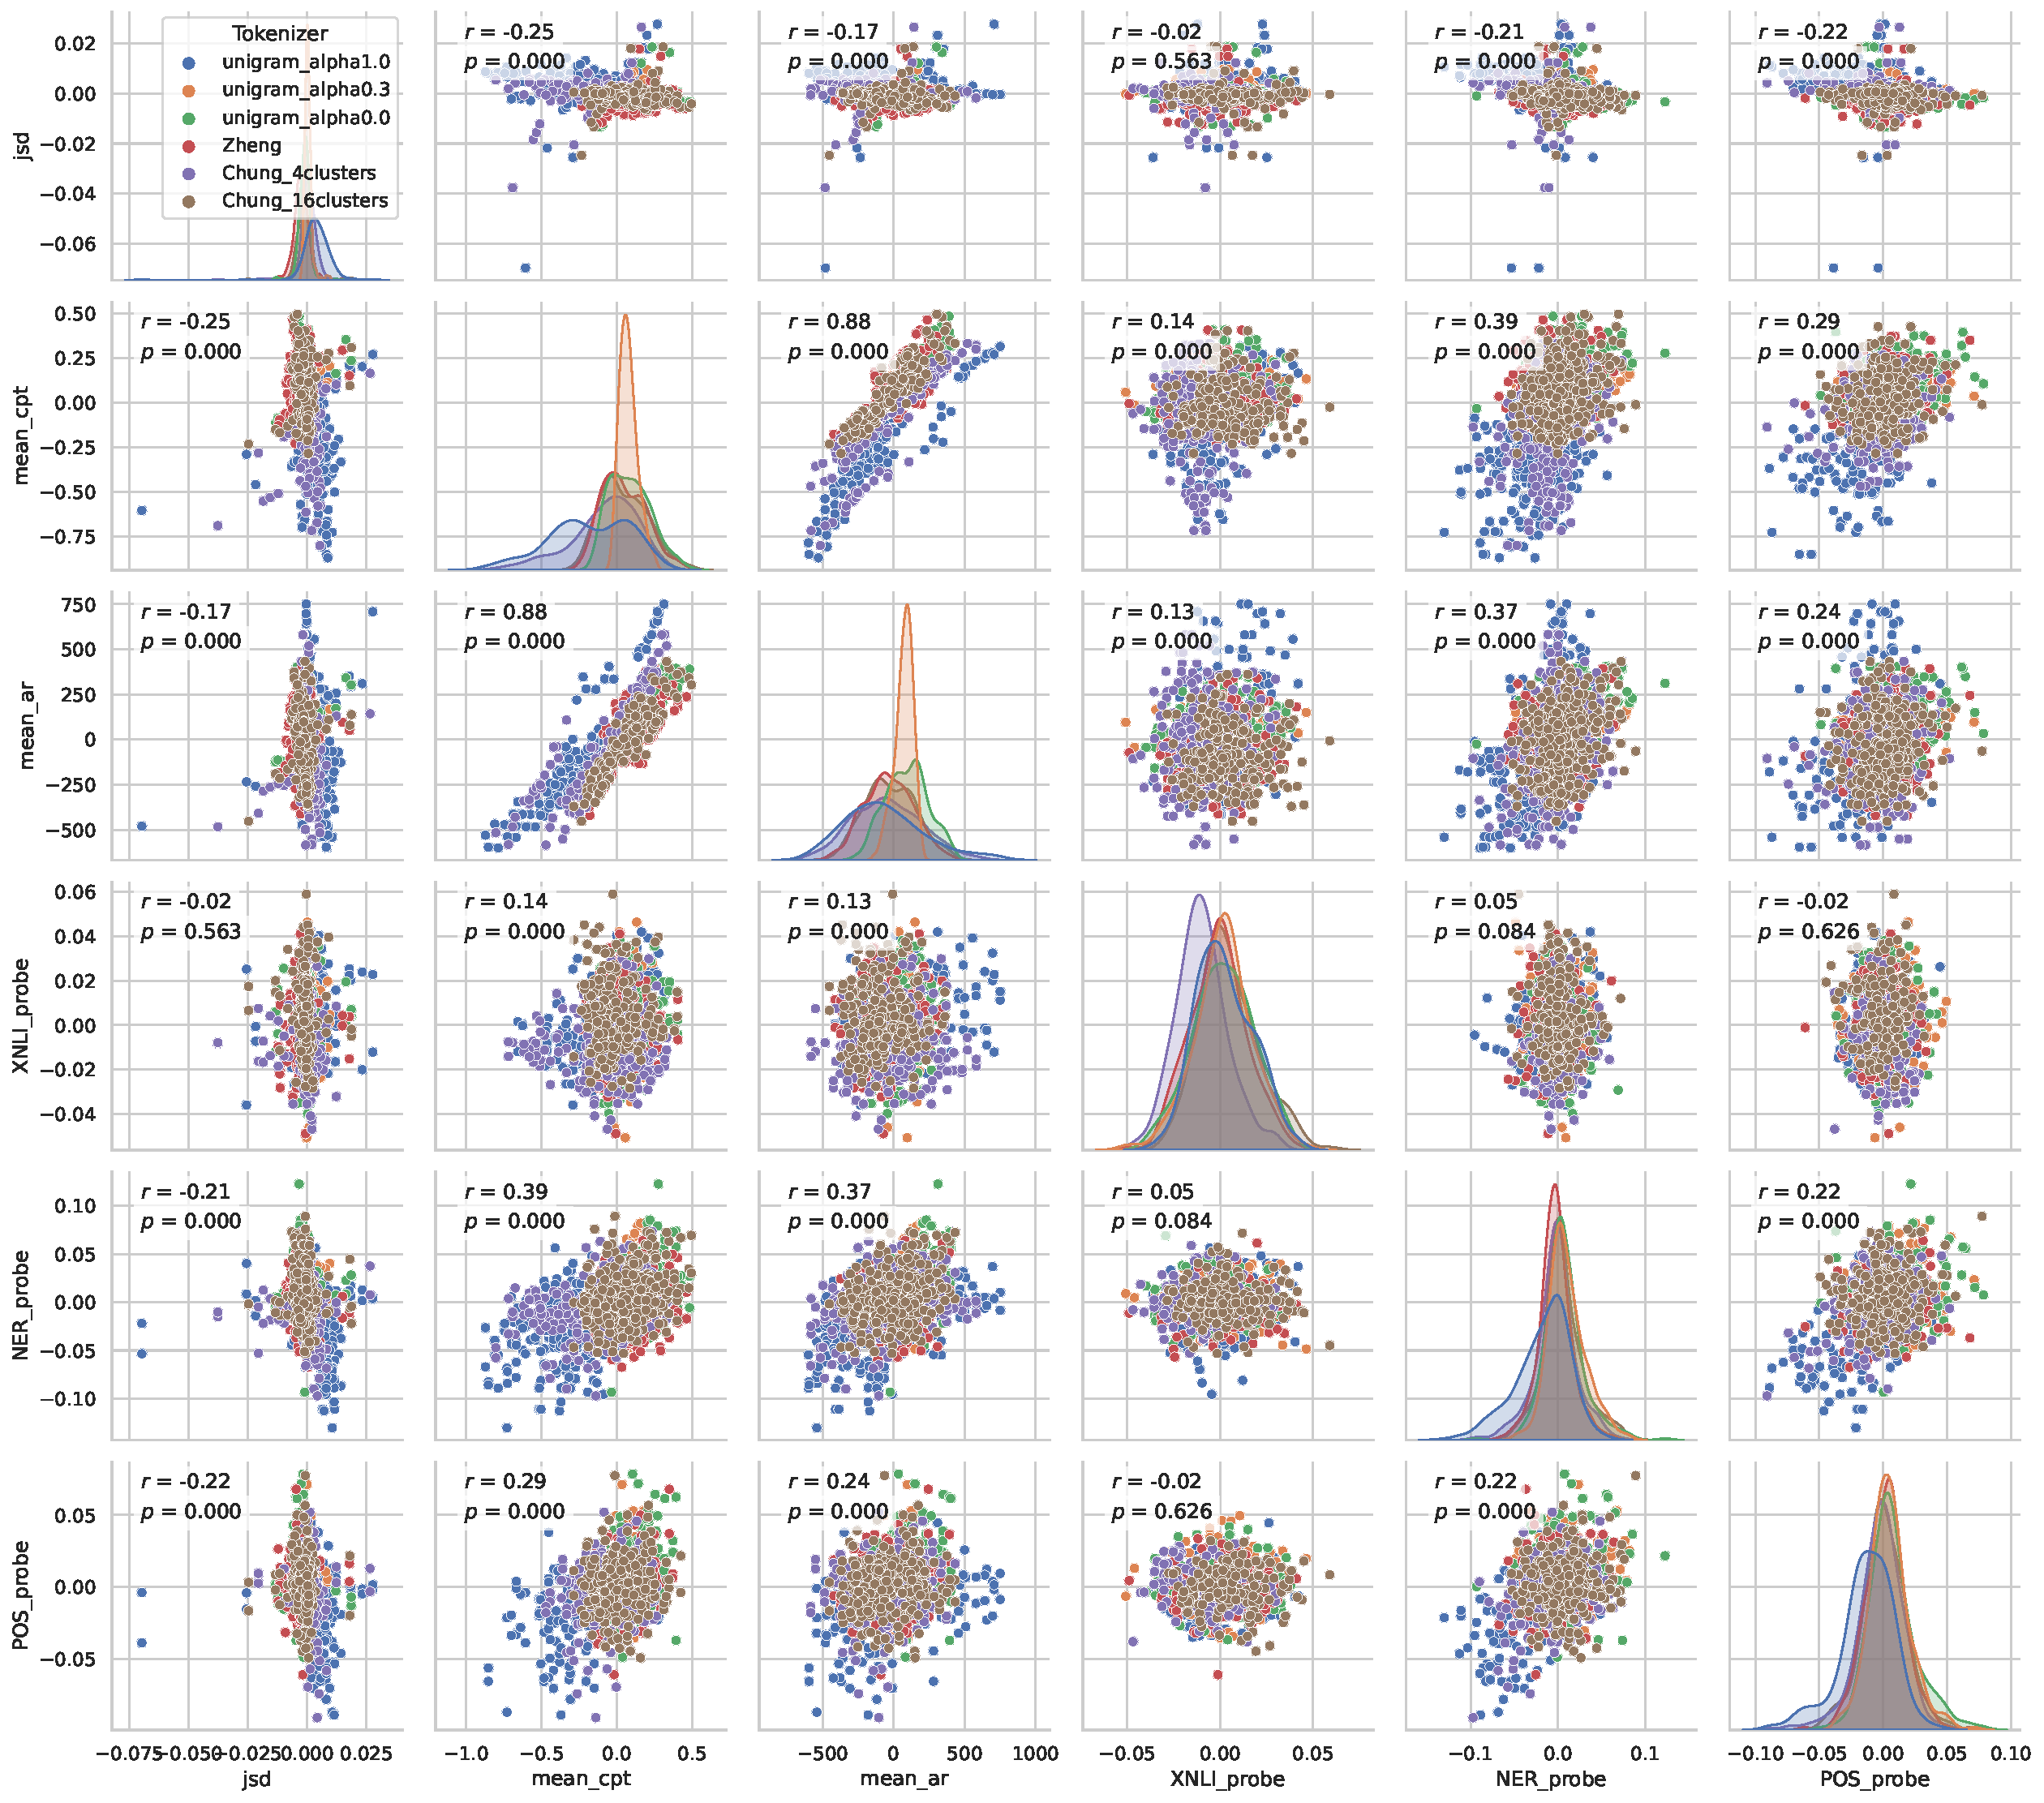
\includegraphics[width=\textwidth]{figures/probe_detailed_crosslanguage_scattermatrix.pdf}
    \caption{We visualize the cross-language results from Figure \ref{fig:probe_overall_crosslanguage} in a scatter matrix. We substract mean performance across the three models from the language pairs results of vocabulary overlap metric (JSD) and the combined CPT/AR of the source and target languages. We see significant, low negative correlations between JSD and F1 scores for the NER and POS tasks and higher, significant correlations between combined CPT and F1 scores. This suggests that the word-level tasks benefit only slightly from an increase in overlap (decrease in JSD) and an increase in token length in source and target languages. For the NLI task, we observe a significant, low correlation between combined CPT/AR and NLI accuracy. This suggests that the cross-lingual transfer for sentence-level tasks benefits very slightly from an increase in allocation in source and target languages.}
    \label{fig:probe_overall_crosslanguage_scattermatrix}
\end{figure}

\section{Findings}

% \textbf{Q4:} What is the effect of using the reproduced methods on the representation of low-resource languages? And
% \textbf{Q5:} How do the reproduced methods compare to the standard method of training the tokenizer on balanced and unbalanced joint corpus?

We find that the balancing methods of \citet{chung_improving_2020,zheng_allocating_2021,liang_xlm-v_2023} improve the representation of low-resource languages by increasing the \textit{vocabulary allocation} for these languages at the cost of lowering the \textit{vocabulary allocation} for the high-resource ones. 

We also find that the Unigram tokenizer trained with a balanced dataset ($\alpha=0.0$) achieves a similar effect as the replicated methods. 

We find a striking similarity between the Unigram tokenizer trained on a balanced dataset and the Zheng method. We find that by maximizing the ALP across languages, Zheng method achieves a similar effect to running an Unigram tokenizer training on a balanced dataset.

We find that the clustering methods with a high number of clusters behave similarly to the Unigram tokenizer trained on a balanced dataset with exceptions of the low-resource languages, that happen to be clustered together with high-resource ones. We assume that the reason is that the clustering methods with a high $k$ are similar to the Zheng method in that they train separate tokenizers for the majority of languages and only a few languages are grouped together.

On the other hand, we find that the clustering methods with lower number of clusters yield more distinct results. Nevertheless, we observe that they are even more susceptible to a decrease in performance when high-resource and low-resource languages are assigned to the same cluster.

By running the extrinsic evaluation, we validate the observations we made using the intrinsic evaluation. We find that the balancing methods improve the word-level tasks for low-resource languages while having no impact on the sentence-level task. 

Interestingly, we also find that the balancing has a net-positive effect for cross-lingual transfer across all languages.

Our findings suggest that in our scaled-down setting of 20 languages and 120k vocabulary size, the simpler method of training a standard Unigram tokenizer on a joint, balanced corpus is sufficient to create a good multilingual vocabulary that represents all languages well.

% Zheng method and the clustering methods with high number of clusters behave similarly


% We observe that the replicated methods of Chung, Zheng, and balanced Unigram do improve the language modeling capabilities over the unbalanced baseline on the word-level tasks while having no impact on the sentence-level task. On the other hand, we do not observe significant differences between the replicated methods and the simple baseline of training the tokenizer on a balanced set which is in line with our previous assessment where we used our proposed tokenizer metrics to arrive at the same conclusion. Our findings suggest that in our scaled-down setting of 20 languages and 120k vocabulary size, the simpler method of training a tokenizer on a joint, balanced corpus is sufficient to create a good multilingual vocabulary that represents all languages well.